\chapter{Introduction}

In the past few decades, with the rapid development of the Machine Learning and Deep Learning, the application of these technologies has become increasingly prosperous worldwide. However, at the same time many data scientists have found: Even examples have only subtle different from the truly examples drawn from the data distributions, they might also be misclassified by particular deep learning models. Many previous works attempted to explain these phenomena with their overfitting and nonlinearity, but Goodfellow argued instead that the primary cause of neural networks' vulnerability to adversarial perturbation is their linear nature, moreover their explanation is verified by quantitative results \cite{goodfellow2014explaining} .

In order to resist adversarial perturbation some provious works suggested training on adversarial examples to regularize the model \cite{goodfellow2014explaining}, and using defensive distillation as strategies to vercus perturbation. But limited by the expensive constrained optimization in the inner loop, this method can not efficiently be used in the model training procedure. Later some authors advised a new approach Parseval Networks to improve robustness to adversarial examples \cite{cisse2017parseval}. In this parseval networks, weight matrices of linear and convolutional layers are maintained to be Parseval tight frames, which are extensions of orthogonal matrices to non-square matrices.

For purpose of a better demonstration of the development in robustness against adversarial, specific experimental data comparison of several latest approaches is presented at the end of this work.

\chapter{Related Work}

Since it was discovered from the recently neural networks, that they are vulnerable to adversarial ex-
amples, some previous works attempts to explain it with their high local variations \cite{szegedy2013intriguing}. Later it is inferred from the experimental results that the neural networks do not capture not the true concepts but learn the discriminative data, which is competent to obtain good accuracy \cite{fawzi2018analysis}.

\chapter{Task}

Since the limitation of many individual inputs precision lead to many problems including the sensor respond similarly to an input x than an adversarial example $\tilde{x}$ = x + $\eta$, when the perturbation $\eta$ is always smaller than the threshold for every element. Then according the dot product between the $\tilde{x}$ and $\omega$ (weight vector): $\bf \omega ^ \top \tilde{x} = \omega ^ \top x + \omega^\top\eta$ and $\bf ||\eta||_\infty < \epsilon$, normally we can through $\eta = sign(\omega)$ to maximize the max norm constraint on $\eta$, and let n, m replace dimensions and the average magnitude of the weight vector $\omega$, then wen can obtain the activation $\epsilon nm$. According to the above procedure many infinitesimal changes of high dimensional problems are finally converted to one large variation by deep learning networks.

The following image is a sufficient demonstration on ImageNet perturbed by the small changes that were the indistinguish difference in the human eyes. In this experiment we set our $\epsilon$ is 0.007 based on the real number of the smallest bit of an 8 bit picture encoding by the conversion of GoogLeNet, then add an imperceptibly small vactor on the correctly panda image which can correctly classified by GoogLeNet as "panda" with confidence 57.7\%, to generate the adversarial example that in the human eye basically is no different from the original image. However the GoogLeNet misclassfies the adversarial example as "gibbon" as well as significantly confidence 99.3\%. Obviously this vulnerability exist also in other different models including shallow softmax classifier, maxout network as well as convolutional maxout network, for these models we have used MNIST test set, ImageNet and preprocessed version of the CIFAR-10 test set, similarly models have extremely high error rates and average confidences.

\begin{figure}
  \begin{center}
    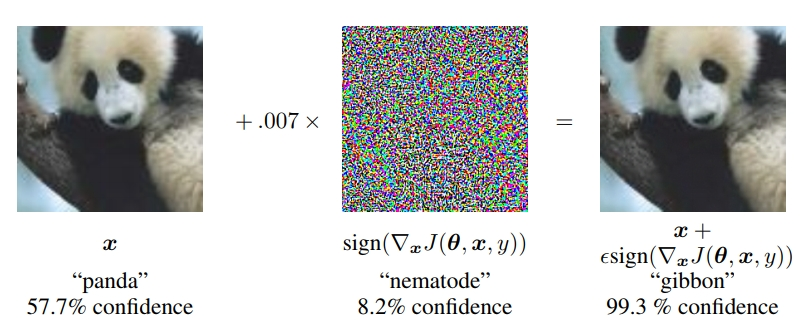
\includegraphics[width=10cm]{image/task.jpg}
  \end{center}
  \caption{ A demonstration of fast adversarial example generation applied to GoogLeNet \cite{szegedy2013intriguing} on ImageNet.}
\end{figure}

The explanation and importance of the vulnerability of the state-of-the-art neural networks against imperceptibly small perturbation was also the primary cause of the rapid development of many useful ways against adversarial examples.

\chapter{Approaches}
\section{Previous Approach: Adversarial Training}

With the discovery of the linear perturbation, the first strategy adversarial training is suggested to improve the robustness of deep networks \cite{goodfellow2014explaining}. In this strategy we have to first define the "first gradient sign method" to generate the adversarial example, so we set $\theta$ be models parameters, and x be the model's input, y replace the targets corresponding to x (for deep learning learning tasks that have targets), last let $J(\theta, x, y)$ refer to the cost used to train the neural network. Finally through the cost function of linearization around the current value of $\theta$ deduce an optimal maximal normalization constrained perturbation:  

$$\eta = \epsilon sign(\nabla_x J(\theta,x,y))$$  

By using this method can man speed up adversarial training. Then the author found an effective regularizer training deep networks with an adversarial objective function which is deduced from the above fast gradient sign method:

$$ \tilde J(\theta,x,y) = \alpha J(\theta,x,y) + (1 - \alpha)J(\theta,x + \epsilon sign(\nabla_xJ(\theta,x,y))$$.

In the experiments, the author first using the dropout to regularize the maxout network, then by adversarial example generated from above algorithm trainging the maxout network with $\alpha$ = 0.5. Of course they get the 0.1\% reduction of the error rate with the adversarial training. Early on the adversarial training set models never able to reduce the error rate to zero. Then using more units per layer like using 1600 units rather than 240 and early stopping when validate the adversarial set.In five different training examples finally generate the result of the dropout masks including four trials error rate is 0.77\% on the test datasets and one trial's error rate is 0.83\%. Before the best reported result is the average value 0.782\% on MNIST, even by fine tuning DBMs with dropout obtain the result of 0.79\%.
 
Adversarial training also make the error rate of the same model on adversarial examples generated by fast gradient sign method from original 89.4\% fell to 17.9\%, and the adversarially trained model on the other hand shows the greater ability to resist the transferable of adversarial examples between different models. However there still exist one unsolvable problem, the confidence of the misclassified an adversarial examples predictions by adversarially trained model is significant high as always, in the paper's experiments 81.4\% of the average confidence on an incorrect example.

Further they also attempt using the scaled gradient's addition or small rotation rather than fast gradient sign method to generate the adversarial examples, however by this new process obtain no special powerful regularizing result. But there are also an inconsistently results from early experiment \cite{szegedy2013intriguing}, in their report using the adversarial perturbation to the hidden layers is the best regularization. Later man put forward another view by the experiment training maxout networks through the hidden layers rotational perturbations: adversarial training  is only useful to the model which have enough capacity to learn against adversarial perturbation, and man never obtained the best results when using perturbations of the final hidden layer in training procedure \cite{goodfellow2014explaining}.

\section{State-of-the-art Approach: Parseval Networks}

The early primary strategies focus on the defensive distillation \cite{papernot2016distillation}, various regularization procedure \cite{gu2014towards}, as well as data augmentation, but complement the regularization by data augmentation like Parseval network shows the improvement of the robustness than them in isolation.

\subsection{Data Augmentation}
The basic process in this step is similar to the previous approach.

1. Adversarial examples

First define the adversarial example is the input pattern $\tilde{x} = x + \delta_x$ where let the train or test input example (x, y), and $\delta_x$ is imperceptibly small so $\tilde{x}$ is also indistinguishable from x. Of course, this example is predicted by the neural network incorrectly. Then give the adversarial example's formally definition:

$$\tilde{x} = \underset{\tilde{x}:||\tilde{x}-x||_p \leq \epsilon}{argmax} l(g(\tilde{x},W),y)$$

where g(.,W) refer the parameters and structure of the network, and p is the normalization type. By taking the first order taylor expansion to compute $\delta_x$ through: 

$$\tilde{x} = \underset{\tilde{x}:||\tilde{x}-x||_p \leq \epsilon}{argmax} (\nabla_x l(g(\tilde{x},W),y))^\top(\tilde{x}-x)$$

Then obtain the first gradient sign method $\tilde{x} = x + \epsilon sign(\nabla_x l(g(\tilde{x},W),y))$ where p = $\infty$, if the p = 2, obtain $\tilde{x} = x + \epsilon \nabla_x l(g(\tilde{x},W),y)$.


2. Generalization with adversarial examples

$$L(W) = \underset{(x,y)\sim D}{\mathbb{E}} [l(g(x, W),y)],$$

$$L_{adv}(W,p,\epsilon) = \underset{(x,y)\sim D}{\mathbb{E}} [\underset{\tilde{x}:||\tilde{x}-x||_p \leq \epsilon}{max} | l(g(\tilde{x}, W),y) - l(g(x, W),y)],$$

There are two interesting generalization errors in the adversarial examples. Then because of the L(W) $\leq L_{adv}$ where p and $\epsilon$ > 0, we obtain:

$$L_{adv}(W,p,\epsilon) \leq L(W) + \underset{(x,y)\sim D}{\mathbb{E}} [\underset{\tilde{x}:||\tilde{x}-x||_p \leq \epsilon}{max} | l(g(\tilde{x}, W),y) - l(g(x, W),y)] \leq L(W) + \lambda_b \Lambda_b \epsilon.$$

Using Lipschitz constant of the neural networks to control the difference between the generalization performance and the average loss value in training process. So we have the formula:

$$ L(W) \leq {1 \over m} \sum_{i=1}^{m} l(g(x_i,W),y_i) + \lambda_p\Lambda_p\gamma + M \sqrt{{2YC_p(\chi, {\gamma \over 2})ln(2) - 2ln(\delta)}\over m}$$.

With the exponential increase of p-norm with $R^D$ the best way is to control the Lipschitz constant g to resistant the adversarial examples.

3. Lipschitz constant of the neural networks

According to the above equations, we obtain $\Lambda_p^{(n,n')}$ definition:

$$||n(x)-n(\tilde{x})||_p \leq \sum_{n':(n,n')\in E} \Lambda_p^{(n,n')}||n'(x) - n'(\tilde{x})||_p$$,

Taking for $\Lambda_p^{(n,n')}$ any value greater than the upper bound of Lipschitz constant $x_0 \in \chi$ for $||.||_p$ 

so the $\Lambda_p^{(n)}$ satisfies:

$$\Lambda_p^{(n)} \leq \sum_{n':(n,n')\in E} \Lambda_p^{(n,n')} \Lambda_p^{(n')}$$

Thus, with the growth of the network's depth the Lipschitz constant increase exponentially. Then for the Linear layers, has n(x) = $W^{(n)}n'(x)$ where $W^{(n)}$ (matrix norm) induced by $||.||_p$, usually definition of $||W^{(n)}||_p$ is:  

$$||W^{(n)}||_p = \underset{z:||z||_p = 1}{sup} ||W^{(n)}z||_p$$

For Convolutional layers, we first defined U(z) where U refers to an unfolding operator, and let z be the input prepared by U, and input's length T, $d_{in}$ replace the inputs channels, so the j-th column is:

$$U_j(z) = [z_{j-k};...;z_{j + k}],$$

Define the convolutional layer of  $d_{out}$ (output channels):

$$n(x) = W^{(n)} * n'(x) = W^{(n)}U(n'(x))$$

and where $W^{(n)}$ refers to a $d_{out} \times(2k+1)d_{in}$ matrix, so deduced $\Lambda_2^{(n)} \leq ||W||_2||U(n'(x))||_2$, also for convolutional layer: $\Lambda_{\infty}^{(n)} \leq ||W^{(n)}||_{\infty} \Lambda_{\infty}^{(n')}$ . For Aggregation layers/transfer functions:, first $\Lambda_p^{(n)} \leq \sum_{n':(n,n')\in \epsilon} \Lambda_p{(n')}$ where we sum up the n nodes inputs and obtain $\Lambda_p^{(n,n')} = 1$, If layer n is transferable, since $\Lambda_p^{(n)} \leq \Lambda_p^{(n')}$, then their Lipschitz constant is $\leq$ 1.

\subsection{Parseval Networks}

Parseval Networks is a regularization scheme improve the robustness of the deep neural networks against adversarial perturbations, in each hidden layer we constrain the Lipschitz constant keep smaller than 1, then we can make the assumption their children nodes Lipschitz constant will keep smaller than 1 too, so successful prevent the Lipschitz constant's exponential growth. Finally at the last layer we can use weight decay or other normal regularization scheme to control the neural network's Lipschitz constant \cite{cisse2017parseval}.

1.Parseval Regularization

The first primary operation in this part is orthonormality of weight matrices, in this procedure we have to maintain the spectral norm of the weight matrix at 1. Moreover, we have to keep the rows of the matrix orthogonal to compute the largest weight matrices singular value in a SGD optimizer. Define the I refers to the identity matrix, then maintains $W^\top W \approx I_{d_{out}\times d_{out}}$. Generally, we constrain the matrix $W\in \mathbb{R}^{d_{out} \times (2k+1)d_{in}}$ of convolutional layers to become a Parseval tight frame, so to keep all singular value of W to $(2k+1)^{(-{1 \over 2})}$, and $\Lambda_2^{(n)}\leq \Lambda_2^{(n')}$ for input node n'. In order to control the weight matrix's $||.||_{\infty}$ and the spectral norm by the normatization of individual rows, we maintaining all weight matrices rows orthogonal. So by rescaling the rows keeping the 1-norm small we successfully completed the improvement of robustness against $||.||_{\infty}$. 

Furthermore, aggregation layers only take a convex combination: $n(x) = \sum_{n':(n,n')\in\epsilon} \alpha^{(n,n')}n'(x)$ with $\sum_{n':(n,n')\in \epsilon}\alpha^{(n,n')}=1$ and $\alpha^{(n,n')} \geq 0$, and the children will appear the inequality $\Lambda_p^{(n)}\leq1$.


2.Parseval Training

Orthonormality constraints is the first significant improvement of Parseval networks on the weight matrices. The difficult part of this operation is to ensure remaining in the manifold after every time updated the parameter, for this we derive an approximate operator by the weight matrices layer-wise regularizer and attempt to guarantee the parseval tightness by this approximate operator, so we have:

$$R_{\beta}(W_k) = {{\beta}\over{2}}||W_k^TW_k - I||_2^2$$

But after every time the update of the gradient descent step, the optimization of $R_{\beta}(W_k)$ and convergence is an extremely expensive process. So we suggest two efficient approximations including perform only once descent on the function $R_{\alpha}(W_k)$ and do the below secondary update after every primary update:

$$ W_k\leftarrow (1+\beta)W_k - \beta W_k W_k^{\top} W_k.$$.

Generally, we have to consider the convexity constraints in aggregation layers. In parseval networks we output not longer the sum up of Residual networks, but the convex combination of their inputs. Let us define the coefficient K-size vector which the layer used for the output of convex combination. For guaranteeing the Lipschitz constant $\Lambda_p^{(n)}\leq 1$ at the node n, after update the gradient we have a euclidean projection of $\alpha$: 

$${\boldsymbol\alpha}^* = \underset{\gamma \in \Delta^{K-1}}{argmin}||\boldsymbol{\alpha-\gamma}||_2^2,$$
where $\Delta^{K-1} = \{\gamma\in\mathbb{R}^K|\boldsymbol{1}^\top \gamma = 1, \gamma \geq 0\}$. Therefore the solution with a soft thresholding operation: 

$$\gamma(\boldsymbol{\alpha}) = {{(\sum_{j\leq k(\alpha)}\alpha_j)-1}\over{k(\boldsymbol\alpha)}}$$

where the sorted coefficients $\alpha_1\geq \alpha_2\geq...\alpha_K$ and $k(\alpha)=max\{k\in(1,......,K)|1+k\alpha_k>\sum_{j\leq k}\alpha_j\}$. In this procedure after every gradient update step we have used the approach \cite{duchi2008efficient} to take the coefficient $\alpha$ projection. 

\chapter{Comparison to previous methods}

\section{ORTHOGONALITY}

\begin{figure}
  \begin{center}
    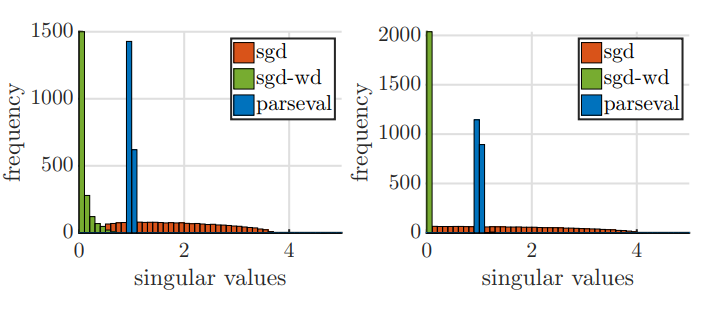
\includegraphics[width=10cm]{image/singular_values_of_the_weight_matrices.png}
  \end{center}
  \caption{Histograms of the singular values of the weight matrices
at layers 1 and 4 of our network in CIFAR-10.}
\end{figure}

Here set the singular value to confirm that Parseval training indeed yields (near)-orthonormal weight matrices. In the experimental evaluation, the singular values obtained with the Parseval Network are tightly concentrated around 1. So this experiment validates that the weight matrices produced by the proposed optimization procedure are orthonormal. But there are many variances in the result of the standard sgd, after adding weight decay come up with a sparse spectrum and demonstrate a low-rank structure in the high layers \cite{denton2014exploiting}.

\section{ROBUSTNESS}

\begin{figure}
  \begin{center}
    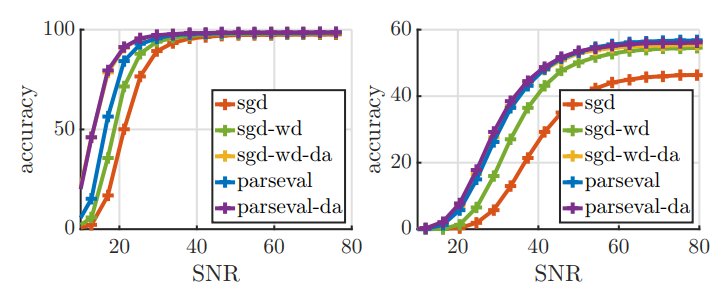
\includegraphics[width=10cm]{image/performance_of_the_models.png}
  \end{center}
  \caption{ Performance of the models for various magnitudes of
adversarial noise on MNIST (left) and CIFAR-10 (right).}
\end{figure}

Through the comparison of figure 3 for Fully connected Nets demonstrate the performance of Parseval networks on both MNIST and CIFAR-10 better than all previous approaches including the adversarial training with weight decay regularization(SGD-wd-da). But even so the combination of adversarial training and Parseval networks (parseval-da) still slightly outperform isolate Parseval networks.

\begin{table}
  \begin{center}
    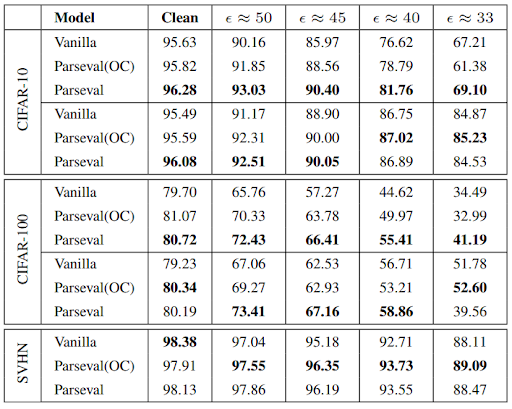
\includegraphics[width=10cm]{image/Classification_accuracy.png}
  \end{center}
  \caption{ Classification accuracy of the models on CIFAR-10 and CIFAR-100 with the (combination of) various regularization scheme. }
\end{table}


Figure 4 shows that on CIFAR-100 for ResNets the combination of Parseval networks, the orthogonality constraint and the convexity constraint outperform Parseval networks combined only the orthogonality.

Thus it is confirmed that the model with Praversal networks obtained significant improvement of robustness against adversarial perturbations, and this depend on efficient controlling the neural networks Lipschitz constant.

\section{CAPACITY}

About 81\% and 56\% at of the whole dimension respectively in the layer 3 and 4 was used by Parseval networks, but SGD-wd-ad has used only 0.4 in the same layer, and the data in Parvesal networks average contract in 30\% and 19\% of the entire dimensions. Thus Parseval makes classification efficient since it contract each class's data in a lower dimensional manifold.

\section{CONVERGENCE}

Due to after each gradient update perform the orthogonalization step, the weight matrices has already conditioned well. So the convergence speed of the Parseval extremely faster than the previous approach.

\chapter{Conclusion}

This paper has illustrated the development of the robustness against adversarial perturbation achieved in recent years, the main focus of this work is on mainstream efficient approaches, including adversarial training and Parseval networks. Furthermore, the comparison of the features between the two models is also presented. Based on the above work, it can be concluded that the robustness of Parseval networks against adversarial noise is more effective than the robustness of all previous approaches.
